\usepackage{graphicx}
\usepackage{makeidx}
\usepackage{alltt}
\usepackage{listings}
\usepackage{polski}
\usepackage{graphicx} 
\usepackage[colorlinks]{hyperref}
\usepackage{tocloft}


\makeindex


	
	

\begin{document}
 
\begin{titlepage}
	\begin{center}
		{\large Uniwersytet Mikołaja Kopernika\\} {\large Wydział Matematyki i Informatyki\\}  \vspace{2.1cm} {\large Łukasz Ogan\\}
		nr albumu: 260196\\
		\vspace{2cm}
		Praca licencjacka\\
		na kierunku informatyka\\
		\vspace{2cm} {\huge Dystrybucje Linuxa na systemie Android\\}
	\end{center}
	\hfill
	\begin{minipage}{8cm}
		\vspace{12mm}
		{Opiekun pracy dyplomowej\\
			dr Andrzej Kurpiel\\
			\\}
	\end{minipage}
	\vspace{2cm}
	\begin{center}
		{Toruń 2016\\}
	\end{center}
	\vspace{1.2cm}
	\begin{minipage}{8cm}
		\begin{center}
			Pracę przyjmuję i akceptuję \vspace{7mm}
			\newline
			................................................\newline
			\small\emph{data i podpis opiekuna pracy}\newline
		\end{center}
	\end{minipage}
	\begin{minipage}{8cm}
		\begin{center}
			Potwierdzam złożenie pracy dyplomowej \vspace{7mm}
			\newline
			................................................\newline
			\small\emph{data i podpis pracownika dziekanatu}\newline
		\end{center}
	\end{minipage}
\end{titlepage}	 

\lstset{basicstyle=\ttfamily,
 	showstringspaces=false,
 	commentstyle=\color{red},
 	keywordstyle=\color{blue},
 	frame=bt,
 	language=Bash,
 	breaklines=true
 }


\tableofcontents

\chapter*{Wstęp}
\addcontentsline{toc}{chapter}{Wstęp}

Celem pracy dyplomowej jest omówienie zagadnień związanych z dystrybucjami systemu Linux, które można uruchomić na urządzeniach mobilnych opartych o architekturę ARM. Praktyczna część pracy skupia się na wykorzystaniu dystrybucji Linuxa uruchomionej obok systemu Android, która ma posłużyć jako serwer telefonii SIP. Część praktyczna składa się z następujących czynności:

\begin{itemize}
	\item Przygotowanie dystrybucji Debiana na architekturę ARM z wykorzystaniem narzędzia debootstrap.
	\item Utworzenie pliku .img z przygotowaną dystrybucją. 
	\item Zainstalowanie w dystrybucji pakietu miniSipServer.
	\item Przygotowanie skryptów startowych.
	\item Przygotowanie aplikacji na urządzenie mobilne służącej do zarządzania systemem oraz pakietem miniSipServer.
\end{itemize} 


Rozdział pierwszy pracy "Dystrybucje Linuxa na system Android", zawiera omówienie architektury ARM. Opisane zostało zagadnienie emulacji systemu. Z pośród popularnych emulatorów wybrany został emulator QEMU, na którym to została pokazana przykładowa emulacja systemu Debian przeznaczonego na architekturę ARM. W dalszych częściach rozdziału opisywane są metody tworzenia odseparowanego systemu plików. Opisany został program na urządzenie mobilne który realizuje uruchomienie wybranej dystrybucji Linuxa. Komunikacja z uruchomionym systemem w tle może odbywać się poprzez protokół VNC, o którym mowa jest w podrozdziale 1.6. Druga część rozdziału skupia się na dystrybucji Debian. Omówiony został zarys historyczny oraz podstawowe narzędzia administracyjnie. Rozdział kończy się opisem narzędzia deboostrap, które służy do przygotowania wybranej dystrybucji Debiana w katalogu uruchomionego już systemu. 


Rozdział drugi "Protokół SIP", skupia się na omówieniu zasady działania protokołu SIP. Wprowadzone zostają podstawowe pojęcia opisujące protokół oraz wyróżnione zostają jego elementy. W kolejnych rozdziałach opisano dokładne działanie protokołu z uwzględnieniem zrzutu danych protokołu podczas działania. Podrozdział 2.3 przedstawia listę implementacji protokołu SIP w systemie Linux  oraz Android z podziałem na oprogramowanie serwerowe i kliencie. W nawiązaniu do pakietu miniSipServer została pokazana jego instalacja. Koniec rozdziału opisuje rynek telefonii SIP


Rozdział trzeci "Projekt informatyczny AndroidLinuxSIPService", opisuje realizacje praktyczną pracy, której celem jest uruchomienie serwera SIP miniSIPServer na systemie Debian Wheezy 7.0 obok systemu Android oraz przygotowanie aplikacji na system Android do zarządzania dystrybucją i serwerem SIP. Opisane zostały etapy tworzenia projektu oraz jego możliwości. 

\section{Załącznik}

Do pracy dołączono DVD-ROM, na którym znajduje się
\begin{itemize}
	\item Źródła pracy w języku LaTeX,
	\item Plik PDF pracy,
	\item Aplikacja w formacie .apk,
	\item Źródła aplikacji,
	\item Obraz dystrybucji,
	\item Skrypt startowy.
	
\end{itemize}

\chapter{Dystrybucje Linuxa na system Android} 


\section{Procesory - Architektura ARM}

Procesor jest to cyfrowe urządzenie sekwencyjne, które występuje w każdym złożonym układzie elektronicznym. Istnieje podział na ze względu na architektury, czyli wspólne określenie najważniejszych z punktu widzenia budowy i funkcjonalności cech procesora (zbiór reguł). Powszechnie w komputerach stosuje się procesory produkowane przez firmę Intel lub AMD odpowiednio 32 lub 64 bitowe. Jeżeli chodzi o urządzenia mobilne lub komputery zminiaturyzowane to stosuje się procesory oparte na architekturze ARM (Advanced RISC Machine) również odpowiednio 32 lub 64 bitowe. Procesory o architekturze ARM należą do rodziny RISC, są szeroko bardzo często stosowane w systemach wbudowanych ze względu na swoją energooszczędną architekturę. Oprócz telefonów komórkowych procesorów ARM używa się między innymi w dyskach twardych, routerach, kalkulatorach czy odtwarzaczach iPod. Aby móc zainstalować system operacyjnym na urządzeniu, które jest wyposażone w procesor ARM, musimy posiadać system który jest przeznaczony na tą architekturę. Przykładem takiego systemu jest Android, który obecnie dominuje na rynku urządzeń mobilnych. System Linux możemy zainstalować na procesorach ARM które posiadają jednostkę MMU (Memory Managment Unit)\footnote{Marcin Bis - Linux w systemach Embedded, układy pełniące realizacje dostępu do pamięci fizycznej żądanej przez CPU}. Na procesory, które nie mają jednostki MMU istnieje projekt uClinux (czyt. "you see linux").


%----------------------------------------------------------------------------------------

\section{Emulacja}


Mamy do dyspozycji jako system operacyjny Windows lub Linux oparty na architekturze Intel lub AMD i uruchomimy na nim poprzez emulacje inny system operacyjny, który docelowo jest przeznaczony na architekturę ARM.

Scenariusz:\newline
- host: Windows 8 64-bit \footnote{Słowa, adresy, jednym słowem mówiąc dane mieszczą się w najwyżej 64 bitach pamięci} \newline
- gość: Debian 32-bit ARM

Do takiej operacji służy nam wcześniej wspomniana emulacja czyli programowe symulowanie działania określonego oprogramowania lub platformy sprzętowej przez inny system lub na sprzęcie innego typu. Dostępnych jest wiele projektów mających na celu zapewnienie wsparcia dla emulacji konkretnych urządzeń. 
\\
\\
Lista popularnych emulatorów:

\begin{itemize}
	\item VirtualBox
	\item VMWare
	\item KVM (Kernel-based Virtual Machine) 
	\item QEMU  \footnote {QEMU - emulator napisany przez Fabrice Bellarda. Jest Bardzo szybki przez co wyprzedza konkurencje. Niestety jest trudniejszy w obsłudze niż inne emulatory.}
	\item Softgun
	\item SkyEye
	\item ARMWare  
\end{itemize}

Jednym z popularnych emulatorów jest QEMU 
http://wiki.qemu.org/. Jest to szybki emulator, który na bieżąco tłumaczy wykonywany kod maszynowy. Potrafi emulować procesory x86, ppc, arm, sparc, mips.
\\
\newpage
QEMU pracuje w dwóch trybach:
\\

1. Emulacja pełnego systemu - procesora i peryferii

\begin{lstlisting}
$ qemu-system-arm -M versatilepb -kernel zImage.bin
\end{lstlisting}


2. Emulacja interfejsu jądra dla przestrzeni użytkownika - umożliwia uruchamianie pojedynczych programów w systemie o innej architekturze.
Przykład: uruchomienie w systemie o architekturze x86 z zainstalowanym QEMU Busyboxa skompilowanego dla architektury ARM:

\begin{lstlisting}
$ qemu-arm -L /cross-tools \
\end{lstlisting}

Do uruchomienia konkretnej aplikacji potrzebna jest biblioteka standardowa w wersji dla architektury docelowej oraz wszystkie dodatkowe biblioteki, których może wymagać aplikacja. Ścieżkę do bibliotek podajemy po parametrze -L.

Instalacja 	

\begin{lstlisting}
$ apt-get install qemu-system
\end{lstlisting}

Lista obsługiwanych platform (urządzeń)

\begin{lstlisting}
$ qemu-system-arm -M ?
\end{lstlisting}

Analogicznie, do wyświetlenia listy procesorów służy polecenie:
\begin{lstlisting}
$ qemu-system-arm -cpu ? 
\end{lstlisting}

Dla systemów bazujących na architekturze ARM9 (armv5) dobrym wyborem będzie emulowanie przez QEMU urządzenie ARM Versatile. 

W celu uruchomienia przygotowanego w emulatorze systemu na urządzeniu należy:

1. Skompilować wersje jądra z opcjami i sterownikami dla konkretnego urządzenia.
2. Przygotować bootloader dla konkretnego systemu.
3. Przenieść bootloader, jądro oraz system plików na urządzenie, na docelowy typ pamięci.


Uruchomienie emulatora:

\begin{lstlisting}
$ qemu-system-arm -M <platform> -m <ilosc pamieci operacyjnej> <opcje uruchamiania>
\end{lstlisting}
\newpage
Domyślna ilość pamięci operacyjnej to 128MB. Opcje uruchamiania mają za zadanie:

\begin{itemize}
	\item Wskazać jądro systemu operacyjnego.
	\item Ustawić parametry konsoli oraz przekazać parametry do uruchamianego jądra.
\end{itemize}

Wszystkie opcje, wraz z przykładami:
\begin{lstlisting}
$ qemu-system-arm -help
\end{lstlisting}

\newpage 

\section{Emulacja Debiana przeznaczonego na architekturę ARM}


Potrzebne pliki znajdują się pod adresem: https://people.debian.org/~aurel32/qemu/armel/
\newline


Uruchomienie:
\begin{lstlisting}
$ qemu-system-arm -M versatilepb -kernel vmlinuz-2.6.32-5-versatile -initrd \ 
initrd.img-2.6.32-5-versatile -hda debian_squeeze_armel_standard.qcow2 \
-append "root=/dev/sda1"
$ qemu-system-arm -M versatilepb -kernel vmlinuz-2.6.32-5-versatile -initrd \
initrd.img-2.6.32-5-versatile -hda debian_squeeze_armel_desktop.qcow2 \
-append "root=/dev/sda1"
\end{lstlisting}


Sterownik loop w systemie Linux udostępnia urządzenia blokowe /dev/loopX\footnote{Istnieje w systemie plików jako /dev/loop (/dev/loop0, /dev/loop1, ...). Sterownik, którego zadaniem jest udawanie urządzeń blokowych (np. dysk twardy), wykorzystuje do tego zwykły plik}. Sterownik loop umożliwia podłączanie do struktury katalogów zawartości obrazów płyt oraz dysków twardych. Możemy również przygotować obraz systemu.

\begin{lstlisting}
mount -o loop plik.iso /mnt
\end{lstlisting}

Przełącznik -t pozwala nam na wskazanie systemu plików.

\begin{lstlisting}
mount -t <system plikow> plik.iso
\end{lstlisting}

Plik ISO zostaje wtedy podłączony do pierwszego wolnego urządzenia /dev/loopX, które jest montowane na katalogu /mnt. 

W przypadku gdy dysponujemy obrazem całego dysku lub karty SD z partycjami musimy skorzystać z polecenia losetup\footnote{Polecenie losetup służy do kojarzenia urządzeń loop z plikami lub urządzeniami blokowymi} ponieważ polecenie mount spodziewa się pliku w którym struktury systemu plików zaczynają się od początku.

\begin{lstlisting}
losetup -o 21232 /dev/loop obraz.img
mount /dev/loop0 /mnt
\end{lstlisting}

Parametr -o w tym przypadku oznacza adres w bajtach, od którego zaczynają się struktury systemu plików.
Adresy kolejnych partycji można odczytać poleceniem fdisk.

\newpage

\section{Narzędzia linuksowe do tworzenia odseparowanego systemu plików}

System Linux oferuje kilka narzędzi w postaci komend, za pomocą których jesteśmy w stanie stworzyć odseparowany system plików.

chroot (ang. change root) - polecenie, które służy do zmiany głównego katalogu (/). Po zmianie głównego katalogu, w nowym środowisku będą działać procesy potomne. Komenda może być użyta jako narzędzie do ochrony przed atakami, atakujący będzie miał dostęp tylko do wydzielonego fragmentu systemu. Sprawdza się również podczas testowania programów, ponieważ ewentualne szkody nie będą dotyczyły głównego systemu. Polecenia może używać tylko superużytkownik root. Nie jest to jednak metoda, która mogłaby się sprawdzić na serwerach dużych korporacji - w takim przypadku korzysta się z technik wirtualizacyjnych.  


Składnia polecenia\footnote{ Manual - http://linux.die.net/man/1/chroot}:
\begin{lstlisting}
chroot [opcje] katalog [argumenty]

--userspec=USER:GROUP  - uzytkownik i grupa do uzycia

--groups=G_LIST  -lista grup

--help - pomoc

--version - wersja polecenia
\end{lstlisting}
Drugim parametrem jest ścieżka do shella, nie trzeba go używać gdyż domyślnie jest to /bin/sh.

Przykład:
\begin{lstlisting}
chroot /usr/local/fedora/rootfs

\end{lstlisting}


Inną komendą, która  działa podobnie jest pivot\_root. Jest jedna jedna różnica, która polega na tym że po wykonaniu polecenia pivot\_root mamy dostęp do starego systemu plików, który możemy umieścić w wybranym przez nas katalogu.  


Składnia polecenia:
\begin{lstlisting}
pivot_root new_root put_old
\end{lstlisting}
Przykład:
\begin{lstlisting}
cd /new-root

mkdir old-root

pivot_root . old-root

\end{lstlisting}


\section{Uruchomienie dystrybucji Linuxa na telefonie z systemem Android}

Sklep Google Play oferuje aplikacje, za pomocą których możemy uruchomić wybraną dystrybucje systemu Linux 

\begin{itemize}
	\item \textbf{Linux Deploy}\footnote{http://github.com/meefik/linuxdeploy} - Debian, Ubuntu, Arch Linux, Fedora, OpenSUSE, KaliLinux, Gentoo, RootFS (instalacja jako plik lub partycja).
	
	\begin{itemize}
		\item Wspierane systemy plików: ext2, ext3, ext4
		\item Obsługiwane architektury: ARM, x86. Obsługa: SSH, VNC, X, framebuffer. Srodowiska graficzne: XTerm, LXDE, Xfce, GNOME, KDE.
		\item Wspierane języki: Angielski, Rosyjski.
	\end{itemize}
	
	Dostęp do kodu źródłowego: https://github.com/meefik/linuxdeploy. Aplikacja napisana jest w języku Java, wykorzystuje skrypty napisane w Bashu (w tym również polecenie chroot).
	
	Zadaniem programu jest stworzenie obrazu IMG na karcie pamięci, zamontowanie go oraz zainstalowanie na nim wybranej dystrybucji. Do poprawnego działania aplikacja potrzebuje dostęp do root oraz internetu. 
	
	Szacowane czasy instalacji systemu Debian wheezy/armhf na telefonie Samsung Galaxy S II:
	
	\begin{itemize}
		\item Without GUI ~ 0:12 / 260 MB
		\item XTerm ~ 0:14 / 290 MB
		\item LXDE ~ 0:19 / 450 MB
		\item XFCE ~ 0:20 / 495 MB
		\item GNOME ~ 0:55 / 1.3 GB
		\item KDE ~ 1:20 / 1.3 GB
	\end{itemize}
	
	Prędkości zapisuj i odczytu dla określonych systemów plików:
	
	\begin{itemize}
		\item	vfat: prędkość odczytu 14.1 MB/s; prędkość zapisu 12.0 MB/s
		\item	ext2: prędkość odczytu 14.9 MB/s; prędkość zapisu 3.9 MB/s
		\item	ext4: prędkość odczytu 14.9 MB/s; prędkość zapisu 16.6 MB/s
		\item	ext2 (loop): prędkość odczytu 17.0 MB/s; prędkość zapisu 7.4 MB/s
		\item	ext4 (loop): prędkość odczytu 17.2 MB/s; prędkość zapisu 8.8 MB/s
	\end{itemize}
	
	
	\item \textbf{Complete Linux Installer}\footnote{http://linuxonandroid.org/complete-linux-installer/} - Ubuntu 13.04, 13.10, Debian 5 and 8, Kali Linux, Fedora 19, Arch Linux, boot widget.
	
	\item\textbf{ DebianDroid}\footnote{https://github.com/uberspot/DebianDroid} - wykorzystuje pakiet debootstrap do przygotowania dystrybucji Debiana na procesor ARM.
	
\end{itemize}

\section{Komunikacja z wykorzystaniem protokołu VNC}
Po zainstalowaniu aplikacji Linux Deploy, pobraniu wybranej dystrybucji i jej zainstalowaniu jesteśmy w stanie połączyć się z zainstalowaną dystrybucją za pomocą protokołu VNC.

VNC (ang. Virtual Network Computing) jest systemem przekazywania obrazu z wirtualnego lub fizycznego środowiska graficznego. Protokół VNC działa w architekturze klient-serwer. Pakiet jest dostępny na najpopularniejsze systemy operacyjne: Android, Windows, Linux, BSD, Mac OS, Solaris, AmigaOS, SCO, Haiku i inne. Konkurentem dla VNC jest NX, który działa z większą wydajnością. 

Domyślnie VNC korzysta z portów TCP 5900 - 5906, gdzie każdy z portów oznacza odrębną sesje (:0 do :6). Istnieje możliwość konfiguracji programu klienta i serwera do pracy na innych portach. 

Popularnym programem, który implementuje protokół VNC jest wieloplatformowy RealVNC opracowany przez giganta w świecie telekomunikacji AT\&T Laboratories, który jest dostępny na stronie http://realvnc.com/

Oprogramowanie składa się z części klienta i serwera. Po zainstalowaniu pakietu jesteśmy w stanie połączyć się z serwerem VNC, który jest uruchomiony na innej maszynie. Mamy ku temu dwie możliwości:
\begin{itemize}
	\item Poprzez GUI programu VNC Viewer, 
	\item Za pomocą przeglądarki internetowej - podając odpowiedni adres i numer portu, uruchamiany jest wtedy aplet napisany w języku Java, który umożliwia nam sterowanie. 
\end{itemize}   

Inne implementacje VNC:

\begin{itemize}
	\item Tight VNC - darmowa implementacja, 
	\item Apple Remote Desktop - oprogramowanie filmy Apple przeznaczone dla systemów Mac OS X,
	\item Ultra VNC - darmowa implementacja, która umożliwia szyfrowanie połączenia,
	\item x11vnc - serwer VNC pozwalający na kontrolowanie zwykłej sesji X11,
	\item TridiaVNC - zmodyfikowana wersja RealVNC.
\end{itemize}

%----------------------------------------------------------------------------------------

\section{Debian - historia}

Autorem systemu Debian jest Ian Murdock\footnote{Zmarł 28 grudnia 2015}, niemiecki programista. Powstanie systemu datuje się na 16 sierpinia 1993r. kiedy to na grupie com.os.linux.\linebreak development Ian Murdock opublikował Manifest Debiana, który definiował stworzenie otwartej dystrybucji opartej na systemie Linux i licencji GNU. Dystrybucja została zbudowana na postawie SLS. Softlanding Linux System (SLS) to jedna z pierwszych dystrybucji Linixa. Została stworzona w 1992 roku przez Petera McDonalda. Była to pierwsza dystrybucja zawierająca nie tylko jądro, ale i również dodatkowe programowanie. Początkowo Debian rozwijał się wolno, wersja 1.x została wydana w 1996. W późniejszych latach system zaczyna rozwijać się bardziej dynamicznie. W 2002 została wydana wersja 3.0 "Woody", która działa na 11 różnych architekturach sprzętowych. 4 maja 2013 została wydana póki co najnowsza wersja stabilna Debiana 7.0 - Wheezy. Wersja 7.0 umożliwia obsługę wielu architektur jednocześnie (multiarch), pozwala to na instalacje pakietów z wielu architektur na tej samej jednostce oraz uruchamianie 32 i 64 bitowych programów. 

\textbf{Gałęzie dystrybucji}
\newline
Debian jest rozwijany w 3 równoległych gałęziach:

\begin{itemize}
	\item \textbf{stablina} (stable)
	\item \textbf{testowa} (testing)
	\item \textbf{niestablina} (eksperymentalna)
\end{itemize}

%----------------------------------------------------------------------------------------


\subsection{Pakiety}

Pakiet to skompilowane źródła danego programu gotowe do instalacji. Pakiety dla Debiana i dystrybucji bazujących na Debianie, mają rozszerzenie \textbf{.deb}\footnote{Od wersji 0.93 systemu pliki deb są implementowane jako archiwum ar}. Typ MIME pliku .deb to application/vnd.debian.binary-package. Pakiet .deb występuje wraz z instalatorem dpkg, który zapewnia zaawansowaną kontrolę powiązań i zależności pomiędzy poszczególnymi składnikami systemu (programy, biblioteki).
Nazwy plików pakietów binarnych systemu Debian są podporządkowane następującej konwencji: \textit{foo\_VersionNumber-DebianRevisionNumber.deb}
\newline
Pakiet \textbf{.deb} to archiwum \textbf{ar} z trzema plikami:

\begin{itemize}
	\item plik debian-binary, w którym zawarta jest informacja o wersji pakietu,
	\item plik kontrolny control.tar.gz - zawiera zależności pakietu, sumy kontrolne oraz skrypty instalacyjne, 
	\item plik danych data.tar.gz - pliki konfiguracyjne, binarne, biblioteki, dokumentacja. 
\end{itemize}
W pakietach .deb stosuje się również silne kompresujące formaty jak bzip2, lzma, xz.
\newline 

Wypakowanie pakietu \textbf{.deb}
\begin{lstlisting}
root@debian:~# ar xv sudo_1.8.5p2-1+nmu2_i386.deb 
x - debian-binary
x - control.tar.gz
x - data.tar.gz
root@debian:~# 
\end{lstlisting}

\newpage
Podgląd pliku control.tar.gz
\begin{lstlisting}
root@debian:~# tar -tzvf control.tar.gz 
drwxr-xr-x root/root         0 2015-02-16 12:08 ./
-rw-r--r-- root/root      4169 2015-02-16 12:08 ./md5sums
-rw-r--r-- root/root       716 2015-02-16 12:08 ./control
-rw-r--r-- root/root        68 2015-02-16 12:08 ./conffiles
-rwxr-xr-x root/root       453 2015-02-16 12:08 ./postrm
-rwxr-xr-x root/root      1380 2015-02-16 12:08 ./prerm
-rwxr-xr-x root/root       441 2015-02-16 12:08 ./preinst
-rwxr-xr-x root/root      1971 2015-02-16 12:08 ./postinst
root@debian:~# 
\end{lstlisting}

\newline
\newline
Wypakowanie tylko pliku data.tar.gz
\begin{lstlisting}
root@debian:~# ar p sudo_1.8.5p2-1+nmu2_i386.deb data.tar.gz | tar zx
\end{lstlisting}

\subsection{Instalacja pakietów}

Do instalacji pakietów \textbf{.deb} służy wcześniej wspomniane narzędzie \textbf{dpkg}.
\newline

Informacje na temat pakietu
\begin{lstlisting}
root@debian:~# dpkg --info sudo_1.8.5p2-1+nmu2_i386.deb 
new debian package, version 2.0.
size 836432 bytes: control archive=4352 bytes.
68 bytes,     4 lines      conffiles            
716 bytes,    17 lines      control              
4169 bytes,    60 lines      md5sums              
1971 bytes,    75 lines   *  postinst             #!/bin/sh
453 bytes,    28 lines   *  postrm               #!/bin/sh
441 bytes,    20 lines   *  preinst              #!/bin/sh
1380 bytes,    50 lines   *  prerm                #!/bin/sh
Package: sudo
Version: 1.8.5p2-1+nmu2
Architecture: i386
Maintainer: Bdale Garbee <bdale@gag.com>
Installed-Size: 1586
Depends: libc6 (>= 2.11), libpam0g (>= 0.99.7.1), libselinux1 (>= 1.32), libpam-modules
Conflicts: sudo-ldap
Replaces: sudo-ldap
Section: admin
Priority: optional
Description: Provide limited super user privileges to specific users
Sudo is a program designed to allow a sysadmin to give limited root
privileges to users and log root activity.  The basic philosophy is to give
as few privileges as possible but still allow people to get their work done.
.
This version is built with minimal shared library dependencies, use the
sudo-ldap package instead if you need LDAP support for sudoers.
root@debian:~# 

\end{lstlisting}

\newline
Instalacja pakietu
\begin{lstlisting}
root@debian:~# root@debian:~# dpkg -i sudo_1.8.5p2-1+nmu2_i386.deb 
\end{lstlisting}

\newline
Usunięcie pakietu
\begin{lstlisting}
root@debian:~# root@debian:~# dpkg -r nazwa_pakietu
\end{lstlisting}

\newline
Lista zainstalowanych pakietów
\begin{lstlisting}
root@debian:~# root@debian:~# dpkg -l
\end{lstlisting}

\newline
Rekonfiguracja pakietu
\begin{lstlisting}
root@debian:~#  dpkg --configure -a sudo_1.8.5p2-1+nmu2_i386.deb 
\end{lstlisting}

\newline
Narzędzia deweloperskie 

\begin{itemize}
	\item dpkg-source pakuje i rozpakowuje pliki źródłowe pakietu,
	\item dpkg-deb pakuje i rozpakowuje pakiety binarne,
	\item dpkg-gencontrol generuje na podstawie informacji zawartych w plikach źródłowych pakietu, plik control dla pakietu binarnego,
	\item dpkg-shlibdeps obliczają zależności od bibliotek,
	\item dpkg-genchanges czyta drzewo katalogów źródłowych po zbudowaniu pakietu i generuje na tej podstawie plik kontrolny (.changes),
	\item dpkg-buildpackage to skrypt pozwalający na automatyczne zbudowanie pakietu,
	\item dpkg-distaddfile dodaje plik do debian/files,
	\item dpkg-parsechangelog czyta plik z zapisem zmian (changelog) rozpakowanego pakietu źródłowego i tworzy opis zmian.
\end{itemize}

\subsection{APT jako narzędzie do pobierania i instalacji pakietów}

Narzędzie apt-get (część APT) służy to pobierania i instalacji pakietów z uwzględnieniem zależności w bardzo prosty sposób. To przeglądania pakietów i operacji na nich służy polecenie aptitude, jest bardziej zaawansowanym narzędziem od apt-get.

\newline
Instalacja pakietu
\begin{lstlisting}
root@debian:~#  apt-get install nazwa_pakietu
\end{lstlisting}


\newline
Szukanie pakietu
\begin{lstlisting}
root@debian:~#  apt-cache search nazwa_pakietu
\end{lstlisting}

\newline
Update pakietów
\begin{lstlisting}
root@debian:~#  apt-get update
\end{lstlisting}


Miejsca skąd można pobierać pakiety to repozytoria, które dzielimy na oficjalne i nieoficjalne. Lista repozytoriów znajduje się w pliku /etc/apt/sources.list

\newline

Przykładowy wpis z pliku /etc/apt/sources.list
\begin{lstlisting}
deb-src http://ftp.pl.debian.org/debian/ etch main non-free contrib
\end{lstlisting}

deb-src informuja nas o typie archiwum, w tym przypadku są to źródła pakietów, które można ściągnąć i skompilować. Dalszą część wpisu stanowi adres repozytorium oraz nazwa dystrybucji. Po nazwie dystrybucji jest sekcja.


W Debianie wyróżniamy trzy sekcje:
\begin{itemize}
	\item main - w niej znajdują się wszystkie wolne pakiety,
	\item non-free - tutaj znajdują się wszystkie niewolne pakiety, czyli takie, które mają zamknięty kod źródłowy,
	\item contrib - tutaj znajdują się wszystkie pakiety wolne, które zależą od pakietów niewolnych.
\end{itemize}


\subsection{Debootstrap}

Pakiet \textbf{debootstrap}\footnote{http://linux.die.net/man/8/debootstrap, https://www.debian.org/releases/stable/amd64/apds03.html.en} jest narzędziem, które umożliwia przygotowanie wybranej dystrybucji Debiana w podkatalogu uruchomionego już systemu. Proces nie wymaga użycia płyty CD, a jedynie dostęp do domyślnego repozytorium Debiana. 


\newline
Syntaktyka polecenia debootstrap
\begin{lstlisting}
debootstrap [OPTION]... <suite> <target> [<mirror> [<script>]]
\end{lstlisting}

\newline

Przykładowy scenariusz z wykorzystaniem pakietu debootstrap:

Nowy katalog dla Debiana:
\begin{lstlisting}
root@debian:~# mkdir /debian
\end{lstlisting}

\newline

Instalacja pakietu debootstrap z repozytorium:
\begin{lstlisting}
root@debian:~# apt-get install debootstrap
\end{lstlisting}


Instalacja pakietu debootstrap z pliku .deb\footnote{http://ftp.debian.org/debian/pool/main/d/debootstrap/}

\begin{lstlisting}
# ar -x debootstrap_0.X.X_all.deb
# cd /
# zcat data.tar.gz | tar xv
\end{lstlisting}

\subsection{Deboostrap - instalacja dystrybucji}

Instalacje należy rozpocząć od utworzenia katalogu /wheezy-chroot

\begin{lstlisting}
export MY_CHROOT=/wheezy-chroot
cd /
mkdir $MY_CHROOT
debootstrap --arch i386 wheezy $MY_CHROOT http://ftp.pl.debian.org/debian
\end{lstlisting}
Mamy do wyboru następujące architektury: alpha, amd64, arm, armel, hppa, i386, ia64, m68k, mips, mipsel, powerpc, s390, sparc. Po poprawnym wykonaniu polecenia deboostrap dodajemy repozytoria do pliku \newline /wheezy-chroot/etc/apt/sources.list:
\begin{lstlisting}
deb http://ftp.pl.debian.org/debian/ wheezy main contrib non-free
deb-src http://ftp.pl.debian.org/debian/ wheezy main contrib non-free

deb http://security.debian.org/ wheezy/updates main contrib non-free
deb-src http://security.debian.org/ wheezy/updates main main contrib non-free
\end{lstlisting}

Oraz do pliku /wheezy-chroot/etc/network/interfaces adresy IP serwerów DNS\footnote{Adresy DNS Google}:
\begin{lstlisting}
nameserver 8.8.8.8
nameserver 8.8.4.4
\end{lstlisting}

Opcjonalnie można z katalogu w którym znajduje się nowy system zrobić obraz.

\newline
Tworzenie pliku obrazu o rozmiarze 2GB\footnote{Polecenie dd służy do niskopoziomowego kopiowania surowych danych}:
\begin{lstlisting}
dd if=/dev/zero of=plik.img bs=1024 count=2000000
\end{lstlisting}
\newline

Za pomocą polecenia mkfs.ext4 zakładamy system plików na obrazie img.

\begin{lstlisting}
mkfs.ext4 plik.img
\end{lstlisting}

Zamontowanie obrazu:
\begin{lstlisting}
mount -t ext4 -o loop plik.img /mnt
\end{lstlisting}

Przekopiowanie zawartości katalogu /wheezy-chroot: 
\begin{lstlisting}
cp -r /wheezy-chroot /mnt
\end{lstlisting}

Odmontowanie:
\begin{lstlisting}
umount /mnt
\end{lstlisting}


W następnym kroku przystępujemy do zamontowania katalogów: /proc, /dev, /sys.
Ważne jest aby zamontować wyżej wspomniane katalogi, ponieważ:

/proc - zawiera informacje o procesach, za pośrednictwem znajdujących się tam plików jądro udostępnia nam informacje na temat parametrów pracy systemu.
/proc w przeciwieństwie do innych systemów plików przechowywany jest w pamięci, a nie na dysku. 
\begin{lstlisting}
ls /proc
[...]
3647  403   4348  5     588  682  749  86   92   988               
404   44    5020  594   696  75   864  93   99        
[...]
\end{lstlisting}
Każdy katalog, którego nazwa jest liczbą odpowiada  uruchomionemu w systemie procesowi. Liczby te informują o numerze PID procesu. 	


\newline
Sprawdzenie wersji jądra
\begin{lstlisting}
cat /proc/version
Linux version 3.19.5-100.fc20.x86_64 (mockbuild@bkernel02.phx2.fedoraproject.org) (gcc version 4.8.3 20140911 (Red Hat 4.8.3-7) (GCC) ) #1 SMP Mon Apr 20 19:51:16 UTC 2015
\end{lstlisting} 

\newline
Ilość pamięci RAM
\begin{lstlisting}
ls -l /proc/kcore
-r--------. 1 root root 140737477881856 08-07 15:25 /proc/kcore
\end{lstlisting}

\newline
\newpage
Lista partycji
\begin{lstlisting}
cat /proc/partitions	
\end{lstlisting}

Inne informacje zawarte na katalogu /proc:
\begin{itemize}
	\item /proc/cpuinfo - informacje o procesorze
	\item /proc/meminfo - informacje o fizycznej pamięci RAM, obszarze wymiany
	\item /proc/mounts - lista zamontowanych systemów plików
	\item /proc/devices - lista dostępnych urządzeń
	\item /proc/filesystems - wspierane systemy plików
	\item /proc/modules - lista załadowanych modułów
	\item /proc/version - wersja jądra
	\item /proc/cmdline - parametry przekazane do jądra podczas uruchomienia
	\item /dev - katalog zawierający pliki specjalne, które odpowiadają urządzeniom. Pliki urządzeń tworzone są podczas instalacji. (komunikacja niskopoziomowa)
	\item /dev/sdb - dysk twardy
	\item /dev/console  - plik odpowiedzialny za klawiaturę
	\item /dev/cdrom  - plik optycznego nośnika danych, CDROM 
	\item /sys - katalog zawierający pliki systemowe, w których można zmieniać parametry jądra
\end{itemize}
Modyfikacja pliku fstab tak aby katalogi montowały się automatycznie: 

\begin{lstlisting}
echo "proc $MY_CHROOT/proc proc defaults 0 0" >> /etc/fstab
mount proc $MY_CHROOT/proc -t proc
echo "sysfs $MY_CHROOT/sys sysfs defaults 0 0" >> /etc/fstab
mount sysfs $MY_CHROOT/sys -t sysfs
\end{lstlisting}

Montowanie wszystkich systemów plików z fstab:
\begin{lstlisting}
mount -a
\end{lstlisting}

Opcjonalnie kopiujemy pliku hosts i mounts.
\begin{lstlisting}
cp /etc/hosts $MY_CHROOT/etc/hosts
cp /proc/mounts $MY_CHROOT/etc/mtab
\end{lstlisting}

\newline  

Zmiana głównego katalogu plików.

\begin{lstlisting}
chroot $MY_CHROOT
\end{lstlisting}

Jeżeli uruchamiamy system który jest w innej architekturze niż komputer hosta konieczne jest dokończenie instalacji. 

\begin{lstlisting}
/debootstrap/debootstrap --secondstage
\end{lstlisting}

Istnieje również pakiet o nazwie dchroot\footnote{http://linux.die.net/man/1/dchroot}, który umożliwia uruchomienie programu, który jest zainstalowany w systemie do którego mamy dostęp za pomocą chroot.

Montowanie partycji
\begin{lstlisting}
root@debian:~# apt-get install dchroot 
\end{lstlisting}

\newline

Konfiguracja - plik /etc/dchroot.conf dodajemy 1 linie
\begin{lstlisting}
x64 /wheezy-chroot
\end{lstlisting}

\newline

Uruchomienie programu w chroot za pomocą dchroot
\begin{lstlisting}
root@debian:~# dchroot -c i386 -d nazwa_programu
\end{lstlisting}

\afterpage{\null\newpage}

\chapter{Protokół SIP}


SIP (Session Initiation Protocol) to protokół drugiej warstwy modelu OSI, który działa w architekturze klient-serwer opisany w dokumencie RFC3261\footnote{https://www.ietf.org/rfc/rfc3261.txt}. Dokument można znaleźć na stronach organizacji IETF (Internet Engineering Task Force). Jego zadanie to inicjowanie sesji pomiędzy jednym lub wieloma klientami,
pozwala również na modyfikacje i zakończenie sesji. Uściślając, główne zadanie protokołu to dostarczenie zestawu funkcji obsługi połączenia. Obecnie jest to dominujący protokół sygnalizujący dla telefonii Voice over IP. Nie jest protokołem transportowym, dlatego konieczne jest jednoczesne zastosowanie protokołu RTP. SIP jest alternatywą dla H.323. Pomysłodawcami protokołu są: M. Handley, H. Schulzrinne, E. Schooler i J. Rosenberg 

Protokół składa się z 2 komponentów:

\begin{itemize}
	\item user agents - użytkownicy
	\item network agents - serwery sieciowe
\end{itemize}
User agent (UA) jest punktem końcowym, może odbierać i ustanawiać połączenia. User agent client (UAC) inicjuje żądania SIP. Serwer user agent server (UAS) odbiera żądania od UAC i zwraca odpowiedź do usera. 

SIP obsługuje pięć funkcji połączenia i zakończenia komunikacji

\begin{itemize}
	\item lokalizacja użytkownika - określenie systemu końcowego, który będzie wykorzystywany do komunikacji
	\item dostępność użytkownika - sprawdzenie gotowości użytkownika, który ma być wywołany do komunikacji
	\item możliwości użytkownika - lista parametrów użytkownika 
	\item połączenie sesji - dzwonienie, zestawienie sesji po obu stronach połączenia
	\item zarządzanie sesją - modyfikowanie parametrów sesji
	
\end{itemize}

SIP można zdefiniować jako komponent, który można użyć z innymi protokołami IETF aby zbudować kompletną architekturę multimedialną. Należy tutaj wymienić protokoły takie jak Real-time Transfer Protocol (RTP) dla transportu danych w czasie rzeczywistym i dostarczania informacji o QoS (jakości usług). Kolejnym protokoły to Real-Time Streaming protocol (RTSP), który wykorzystywany jest do sterowania strumieniem medialnym, Media Gateway Control Protocol (MEGACO) wykorzystywany do sterowania bramami w sieci publicznej PSTN oraz Session Description Protocol (SDP) dla opisania sesji.

Protokół dostarcza również szereg usług bezpieczeństwa, które między innymi chronią przed atakami DOS (denial-of-service), dbają o uwierzytelnienie, chronią integralność, oferują możliwość szyfrowania. SIP jest kompatybilny z protokołem IPv4 oraz IPv6.

\begin{figure}[H]
	\centering
	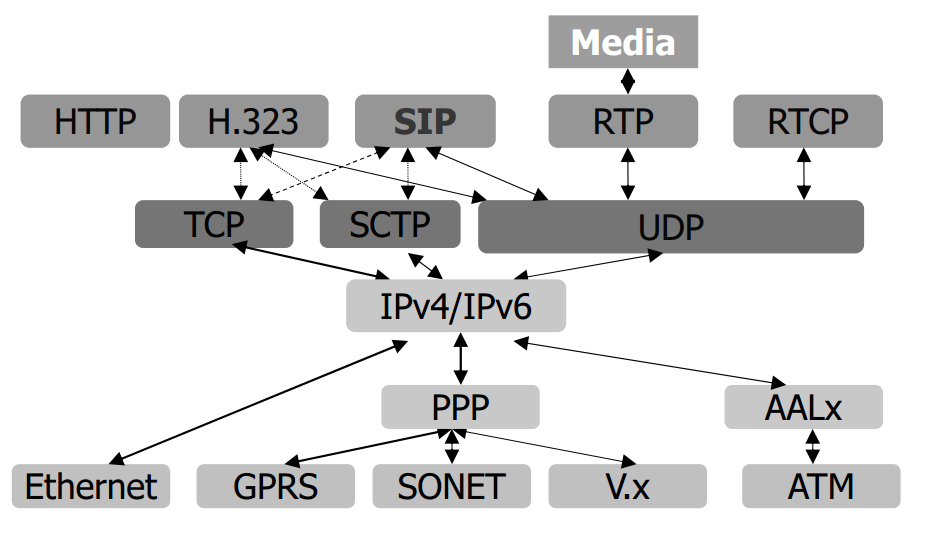
\includegraphics[width=0.7\linewidth]{sip_stos_proto}
	\caption{Stos protokołów}
	\label{fig:sip_stos_proto}
\end{figure}

\section{Elementy sieci SIP}

Terminale końcowe (nodes) to aplikacje uruchamiane na komputerze lub na aparatach telefonicznych, które używają protokołu SIP i RTP.

Rejestrator SIP (registrar) baza danych, która komunikuje się z węzłami SIP w celu zbierania i archiwizacji informacji na temat użytkowników SIP. Zebrane dane są wykorzystywane w trakcie nawiązywania połączenia do odnajdowania w sieci węzłów docelowych.

Połączenia SIP, które nie są lokalne muszą być przekazywane przez serwery pośredniczące SIP proxy. 



\section{Działanie protokołu SIP}


Dzwoniący do siebie użytkownicy stosują identyfikacje SIP URI (Uniform Resource Identifier). Adres wygląda następująco:
\begin{lstlisting}
uzytkownik@domena:port
\end{lstlisting}
Gdzie korzysta się z domyślnego numeru portu 5060.
SIP jest podobny do protokołu HTTP, dzieli z nim wiele zasad konstrukcyjnych między innymi używa zwykłego tekstu i wykorzystuje mechanizm żądanie-odpowiedź. SIP jest w stanie zagwarantować bezpieczne, szyfrowane połączenie TLS (Transport Layer Security) SIPS URI. Protokół zbudowany jest warstwowo co oznacza, że jego zachowanie jest opisane przez niezależne stany przetwarzania z luźnym powiązaniem między poszczególnymi stanami (stadiami). Najniższą warstwą SIP jest składnia i kodowanie, które wykonywane jest przy użyciu gramatyki BNF (Backus-Naur Form). Warstwa transportowa plasuje się na drugim miejscu w hierarchii. Jej zadanie to określenie w jaki sposób klient wysyła żądania i otrzymuje odpowiedzieć oraz jak serwer wysyła/odbiera żądania/odpowiedzi poprzez sieć. Trzecia warstwa to warstwa transakcyjna. Transakcja jest żądaniem wysyłanym przez transakcje klienta do transakcji serwera, z wszystkimi odpowiedziami na żądanie, wysłanymi z transakcji serwera do klienta. Warstwa obsługuje retransmisje warstwy aplikacyjnej, dopasowanie odpowiedzi do żądań. Ostatnia warstwa to warstwa użytkownika transakcji. Każdy z użytkowników jest użytkownikiem transakcji. 




Protokół SIP korzysta z następujących metod:

\begin{itemize}
	
	\item INVITE - zapoczątkowanie wywołania przez zaproszenie użytkownika do sesji
	\item ACK - potwierdza odebranie odpowiedzi na żądanie INVITE
	\item BYE - zakończenie wywołania
	\item CANCEL - anulowanie żądania trwającego
	\item REGISTER - rejestrownie agenta użytkownika
	\item OPTIONS - odpytanie o możliwości serwera
	\item INFO - przenoszenie informacji dodatkowej, np. cyfr DTMF
	
\end{itemize}

Kody odpowiedzi SIP (podobieństwo do kodów odpowiedzi protokołu HTTP):

\begin{itemize}
	
	\item 1xx - Wiadomości informacyjne
	\item 2xx - Odpowiedzi pozytywne
	\item 3xx - Odpowiedzi przekierowania
	\item 4xx - Odpowiedzi błędnych żądań
	\item 5xx - Odpowiedzi błędu serwera
	\item 6xx - Odpowiedzi błędów globalnych
	
\end{itemize}
Wyżej wspomniane metody oraz odpowiedzi używane są do ustanowienia sesji połączenia.


Architektura składa się z następujących elementów:

\begin{itemize}
	\item User Agent Client (UAC)
		\begin{itemize}
			\item systemy końcowe
			\item UAC odpowiedzialny jest za wysyłanie żądań SIP
		\end{itemize}
\end{itemize}

\begin{itemize}
	\item User Agent Server - UAS
	\begin{itemize}
		\item odbiera żądania połączeń
		\item wysyła odpowiedzi 
	\end{itemize}
\end{itemize}

\begin{itemize}
	\item User Agent (terminal)
	\begin{itemize}
		\item UAC oraz UAS
	\end{itemize}
\end{itemize}

\begin{itemize}
	\item Redirect Server
	\begin{itemize}
		\item zajmuje się przekierowaniem użytkownika na inny serwer
	\end{itemize}
\end{itemize}

\begin{itemize}
	\item Proxy Server
	\begin{itemize}
		\item reprezentuje żądanie do innego serwera
	\end{itemize}
\end{itemize}

\begin{itemize}
	\item Registrar
	\begin{itemize}
		\item odpowiedzialny za odebranie zgłoszenia rejestracyjnego
	\end{itemize}
\end{itemize}

\begin{itemize}
	\item Location Server
	\begin{itemize}
		\item baza danych użytkowników 
	\end{itemize}
\end{itemize}

Graficzna reprezentacja została przedstawiona na rysunku 2.2.
\begin{figure}[H]
	\centering
	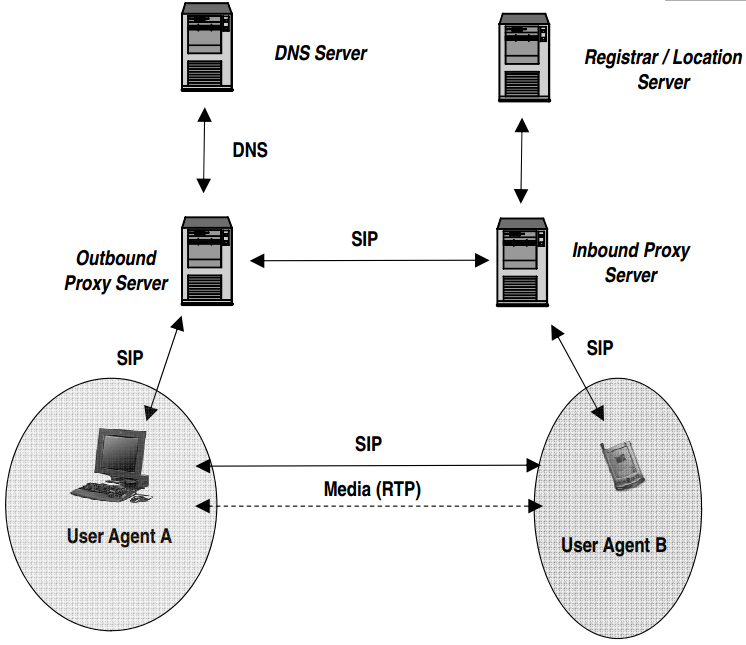
\includegraphics[width=0.7\linewidth]{architektura}
	\caption{Architektura SIP - User Agent}
	\label{fig:architektura}
\end{figure}
\newpage

Nagłówek SIP ma postać tekstową dzięki czemu jest łatwy do odczytania.

\begin{lstlisting}
INVITE sip:UserB@there.com SIP/2.0
Via: SIP/2.0/UDP 4.3.2.1:5060
To: User B <sip:UserB@there.com>
From: User A <sip:UserA@here.com>
Call-ID: 4598998103413@4.3.2.1
CSeq: 1 INVITE
Contact: <sip:UserA@4.3.2.1>
Content
-Type: application/sdp
Content
-Type: application/sdp
Content-Length: 201
v=0
o=UserB 289375749 289375749 IN IP5 100.101.102.103
s=-
c=IN IP4 100.101.102.103
t=0 0
m=audio 5004 RTP/AVP 0
m=audio 53000 RTP/AVP 96
c=IN IP4 200.201.202.203
a=rtpmap:96 telephone-event
\end{lstlisting}

\section{Implementacje protokołu SIP w systemie Linux    - serwery} 

\subsection{miniSipServer}
MiniSIPServer\footnote{https://www.myvoipapp.com/} to profesjonalny, wielopratformowy serwer VoIP. Serwer, do którego można pobrać klienta tej samej firmy o nazwie miniSIPPhone jest oparty o standard SIP. Autorzy oprogramowania zadbali również o to aby system był kompatybilny z urządzeniami, które oparte są na procesorze ARM. 


\subsubsection{Instalacja}
Przed zainstalowaniem serwera SIP, należy zainstalować niezbędne biblioteki. 

\begin{lstlisting}
sudo apt-get install gcc g++ libqt4-dev libqtcore4 libqtgui4 libqt4-network libqt4-xml libssl-dev libmysqlclient18 libmysqlclient-dev python-dev libsrtp0-dev
\end{lstlisting}
Plik: http://www.myvoipapp.com/download/index.html. 

\begin{lstlisting}
sudo dpkg -i mss_pi_u20.deb
\end{lstlisting}
Jeżeli wszystko się powiedzie to pliki serwera znajdą się w katalogu /opt/sipserver/

\subsubsection{Uruchomienie}

Serwer uruchamiamy za pomocą polecenia:
\begin{lstlisting}
/opt/sipserver/msscli&
\end{lstlisting}
Możliwość zarządzania serwerem jest możliwa z poziomu przeglądarki internetowej. W tym celu należy w oknie przeglądarki wpisać własny numer IP i port 8080. 


\subsection{Asterisk}
Najpopularniejszym serwerem wykorzystującym protokół SIP jest Asterisk\footnote{http://www.asterisk.org/}. Jest to kompletne oprogramowanie centrali telefonicznej PBX.
Główne cechy:
\begin{itemize}
	\item dostępny na systemy Windows, Linux, BSD, Mac OS X
	\item obsługa protokołów SIP, IAX, H.323, ADSI, MGCP, SCCP
	\item telekonferencje
	\item poczta głosowa
	\item nagrywanie rozmów
	\item współpraca z bazami danych MySQL, PostgreSQL
\end{itemize}   


\subsection{Cipango}

Rozszerzenie  do popularnego serwera Jetty napisane w języku Java. 
Główne cechy:
\begin{itemize}
	\item łatwość w użyciu
	\item wspiera SIP Servlets oraz HTTP Servlets
\end{itemize}

\subsection{Elastix}

Oprogramowanie przeznaczone na system Linux, opiera swoją funkcjonalność na wspominanym wcześniej Asteriskiem, FreePBX, HylaFAX, Openfire oraz Postfix.

\subsection{FreeSWITCH}

Wieloplatformowe oprogramowanie służące do komunikacji za pomocą dźwięku, wideo oraz tekstu. 
Główne cechy:
\begin{itemize}
	\item wsparcie dla Skype, SIP, H.323, WebRTC
	\item moduł konferencji 
\end{itemize}

\subsection{Kamailio}

Serwer umożliwiający zapewnienie ułatwienie z konfiguracji Asteriska. Za pomocą niego można rozbić konfiguracje na serwer SIP obsługujący rejestracje oraz serwer Asterisk realizujący połączenia. 

\subsection{Inne serwery SIP}
 
\begin{itemize}
	\item 2600Hz blue.box
	\item FreePBX
	\item GNU SIP Witch
	\item Mobicents 
	\item Mysipswitch
	\item OpenSIPS
	\item SailFin
	\item SIP Express Router (SER)
	\item Enterprise Communications System sipXecs
	\item Yate
	\item YXA
\end{itemize}

\section{Implementacje protokołu SIP w systemie Android - serwery}

\subsection{uSipServer}

Prosty w użyciu serwer SIP na system Android, do pobrania ze sklepu Google Play.
 
\section{Implementacje protokołu SIP w systemie Linux - klienty}

\subsection{Blink}
Klient SIP działający w systemach Linux oraz Windows. Napisany w oparciu o bibliotekę Qt. Umożliwia między innymi obsługę wideo, wymianę plików między użytkownikami, udostępnianie pulpitu.  

\subsection{KPhone}
Klient przeznaczony tylko na systemy Linux. Ma zaimplementowaną funkcjonalność telefonu VoIP, ale nie ogranicza się tylko do niego. Wspiera NAT oraz STUN. Obsługuje systemy dźwięku ALSA i OSS. Wykorzystuje protokół SRTP to szyfrowania rozmów głosowych.

\subsection{Linphone}

Program klienta napisany w języku C przez francuską firmę Belledonne Communications. Wspiera dodatkowo system Windows, Max OS X oraz systemu mobilne Windows Phone, iOS, Android. Zapewnia szyfrowanie rozmów z użyciem protokołu ZRTP.

\subsection{Zoiper}
Wieloplatformowe oprogramowanie o szerokiej funkcjonalności. Oferuje wysoką jakość rozmów oraz szyfrowanie ich z wykorzystaniem protokołów SRTP oraz TSL. Występuje również w postaci programu klienta. 

\subsection{Inne klienty SIP}
 
\begin{itemize}
	\item  Ekiga
	\item  Empathy
	\item  Jitsi
	\item  MicroSIP
	\item  QuteCom
	\item  SFLphone
	\item  Telephone
	\item  Twinkle
	\item  Yate client
\end{itemize}

\section{Implementacje protokołu SIP w systemie Android - klienty}

System Android oferuje natywnego klienta SIP\footnote{http://www.voipvoip.com/android/sip.html}. Jest on  dostępny od wersji 2.3 systemu. 
\subsection{Konfiguracja natywnego klienta SIP}
Należy przejść do Ustawień, wybrać ustawienia rozmów i następnie poszukać zakładki Konta. Następnie pojawi się lista kont SIP, aby dodać nowe konto należy wybrać przycisk "Dodaj konto". Na dodanie nowego konta składa się: podanie nazwy użytkownika, hasła, serwera. Po pomyślnym dodaniu konta system jest gotowy do dzwonienia przez internet wykorzystując WiFi. Dzwonienie z wykorzystaniem sieci 3G jest niemożliwe.


\subsection{Sipdroid}
Projekt oparty o dostęp do kodu źródłowego. W najnowszej wersji 3.0 umożliwia szyfrowanie rozmów. Aplikacja oferuje wysyłania VideoSMSów oraz stworzenie darmowego konta PBX ale użytkowników posiadających konto w usłudze Google Voice. Aplikacja pozwala wybrać w jakich sieciach ma korzystać z VoIP (Wi-Fi, 3G, EDGE).

 
\begin{figure}[H]
\centering

\includegraphics[width=0.4\linewidth]{Screenshot_2015-09-21-11-11-11}
\caption{Sipdroid}
\label{fig:Screenshot_2015-09-21-11-11-11}
\end{figure}



\subsection{CSipSimple}
Prosty klient SIP na system Android. Cechuje się wysoką wydajnością i  łatwą konfiguracją. Oferuje nagrywanie rozmów oraz obsługuje kodek HD.

 

\begin{figure}[H]
\centering
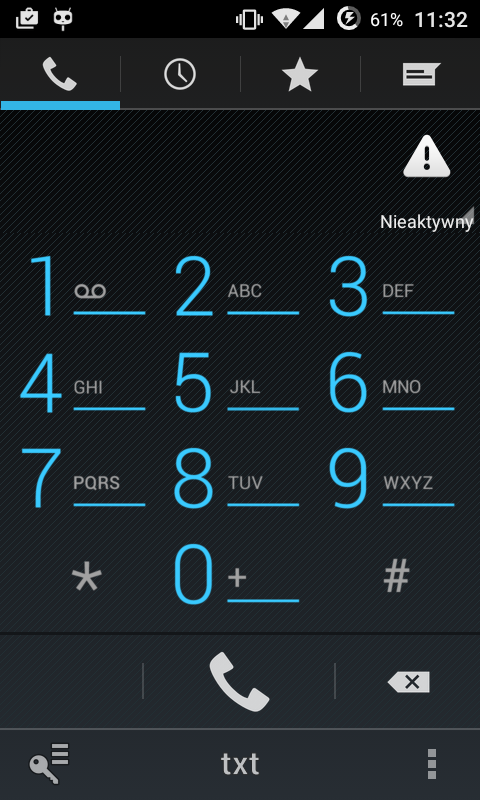
\includegraphics[width=0.4\linewidth]{Screenshot_2015-09-21-11-32-02}
\caption{CSipSimple}
\label{fig:Screenshot_2015-09-21-11-32-02}
\end{figure}



\subsection{Bria VoIP Softphone}
Kolejny klient SIP dostępny w sklepie Google (komercyjny). Zarządzany przez firmę CounterPath Corporation, lidera na rynku produktów i rozwiązań oprogramowania VoIP. Produkt cechuje się wysoko bezpieczną komunikacją między użytkownikami oraz wysoką jakością dźwięku. Konto Premium umożliwia połączenia wideo. Umożliwia połączenia z wykorzystaniem sieci Wi-Fi oraz 3G. 
\newpage


\section{Rynek telefonii SIP}

Jednym z problemów związanym z protokołem SIP, który wchodzi w skład VoIP jest niewłaściwa konfiguracja zapory sieciowej co uniemożliwia zainicjowanie połączenia z zewnątrz. Rozproszona natura protokołu utrudnia spełnienie wszystkich prawnych wymagań nałożonych na operatorów telekomunikacyjnych. Na polskim rynku jest co raz więcej rozwiązań telefonicznych opartych o protokół SIP, oferują je między innymi firmy Orange, HaloNet, Tlenofon, Freeconet, HopIn.pl, INTERFON, IPFON, EuroTC, DigiTEL, Siec T2, Actio, Newfon, easyCALL, PLFON, iFON. Duże firmy telekomunikacyjne takie jak 3Com, Avaya, Cisco oraz Nortel umożliwiają współpracę z sieciami SIP. Na polskim rynku telefonii dla firm najwięcej sprzedaje się klasycznych systemów telefonicznych, ale rozwiązania telefonii IP cieszą się coraz większym zainteresowaniem. Głównymi odbiorcami systemów telefonii IP są firmy średniej wielkości, które zatrudniają 300 - 800 pracowników oraz duże korporacje. Infonetics Research prognozuje, że do 2018 rynek  usług VoIP przeznaczonych dla odbiorów domowych i biznesowych wzrośnie do 88 miliardów dolarów na świecie. Najszybciej rośnie segment hostowanych usług VoIP oraz Unified Communications przeznaczonych dla przedsiębiorstw. Największe przychody w grupie usług biznesowych generują usługi IP PBX. Z usług operatorów VoIP korzystają mieszkańcy Francji, Dani i Niemiec. Polska ma swój udział w około 4 \%.        
\newpage
\afterpage{\null\newpage}
\chapter{Projekt informatyczny AndroidLinuxSIPService}

Celem projektu jest uruchomienie serwera SIP miniSIPServer na systemie Debian Wheezy 7.0 obok systemu Android oraz przygotowanie aplikacji na system Android do zarządzania dystrybucją systemu linux oraz serwerem SIP. Zadanie obejmuje następujące czynności:

\begin{itemize}
	\item przygotowanie dystrybucji systemu Linux na system Android
	\item zainstalowanie środowiska graficznego Xfce na przygotowanej dystrybucji
	\item zainstalowanie programu miniSipServer na przygotowanej dystrybucji
	\item zainstalowanie serwera SSH oraz serwera VNC Tightvnc
	\item przygotowanie skryptów startowych dla SSH i Tightvnc i umieszczenie ich w nowo przygotowanej dystrybucji
	\item uruchomienie przygotowanej dystrybucji razem z serwerem SIP na telefonie z systemem Android
	\item przygotowanie aplikacji na system Android do zarządzania systemem Linux.
\end{itemize}
\newpage

\section{Narzędzia programistyczne użyte do realizacji}


\subsection{Przygotowanie dystrybucji}
Dystrybucja przygotowywana jest za pomocą narzędzia debootstrap.

\begin{lstlisting}
mkdir /home/debian-chroot
debootstrap --arch armhf wheezy /home/debian-chroot http://ftp.pl.debian.org/debian
\end{lstlisting}

Następnie tworzony jest obraz z powstałego katalogu.

\begin{lstlisting}
dd if=/dev/zero of=plik.img bs=1024 count=2000000

mkfs.ext4 debian.img

mkdir /mnt/debian-chroot
mount -t ext4 -o loop debian.img /mnt/debian-chroot

cp -r /home/debian-chroot /mnt/debian-choort
\end{lstlisting}

\subsection{Przygotowanie skryptu}

W następnym kroku przygotowany zostaje skrypt w języku Bash, który ma za zadanie:

\begin{itemize}
	\item zamontowanie przygotowanego obrazu
	\item zamontowanie katalogów /proc, /dev, /sys\footnote{/sys zawiera pliki systemowe w których można zmieniać parametry jądra}, /dev/pts\footnote{/dev/pts to wirtualny system plików, który zawiera informacje o pseudo terminalach}
	\item opcjonalnie uruchomienie serwera SSH i serwera SIP w "nowym systemie" wykorzystując polecenie chroot i skryptów startowych
	\item zatrzymanie uruchomionych usług
	\item odmontowanie katalogów /proc, /dev, /sys, /dev/pts
	\item odmontowanie przygotowanego obrazu
\end{itemize}

\subsection{Wybór serwera SIP}
Jako serwer SIP wykorzystywany jest wcześniej wspominany miniSipServer w wersji 22. miniSipServer jest wieloplatformowym serwerem. Firma udostępnia również dystrybucje na procesory ARM, dedykowaną na Raspberry Pi. Serwer ten został wybrany ze względu na stabilność działania na systemie w architekturze ARM.
\subsection{Przygotowanie aplikacji na system Android}
Aplikacja na system Android została przygotowana w środowisku Android Studio\footnote{http://developer.android.com/intl/es/tools/studio/index.html}, które jest oparte na Intellij\footnote{https://www.jetbrains.com/idea/ - IDE do programowania w języku Java firmy JetBrains, której środowiska uważane są za najlepsze na rynku}. Jest to kompletne środowisko programistyczne, wszystko jest w jednym miejscu. Bogata funkcjonalność zwalnia nas z ciągłego testowania kodu poprzez kompilacje. Aplikacja wymaga do pracy jedynie bibliotek JDK. SDK Andoirda pobierane jest automatycznie w razie potrzeby. Za pomocą specjalnego managera można zarządzać zainstalowanymi składnikami. Interfejs aplikacji jest bardzo intuicyjny. Układ elementów i okien jest konfigurowalny. Powyższe zalety zadecydowały na skorzystaniu z Android Studio. Do wyboru na rynku jest jeszcze środowisko Eclipse\footnote{https://eclipse.org/} z wtyczką ADT. 
Interfejs aplikacji prezentuje rysunek 3.1.
\newpage
\begin{figure}[H]
	\centering
	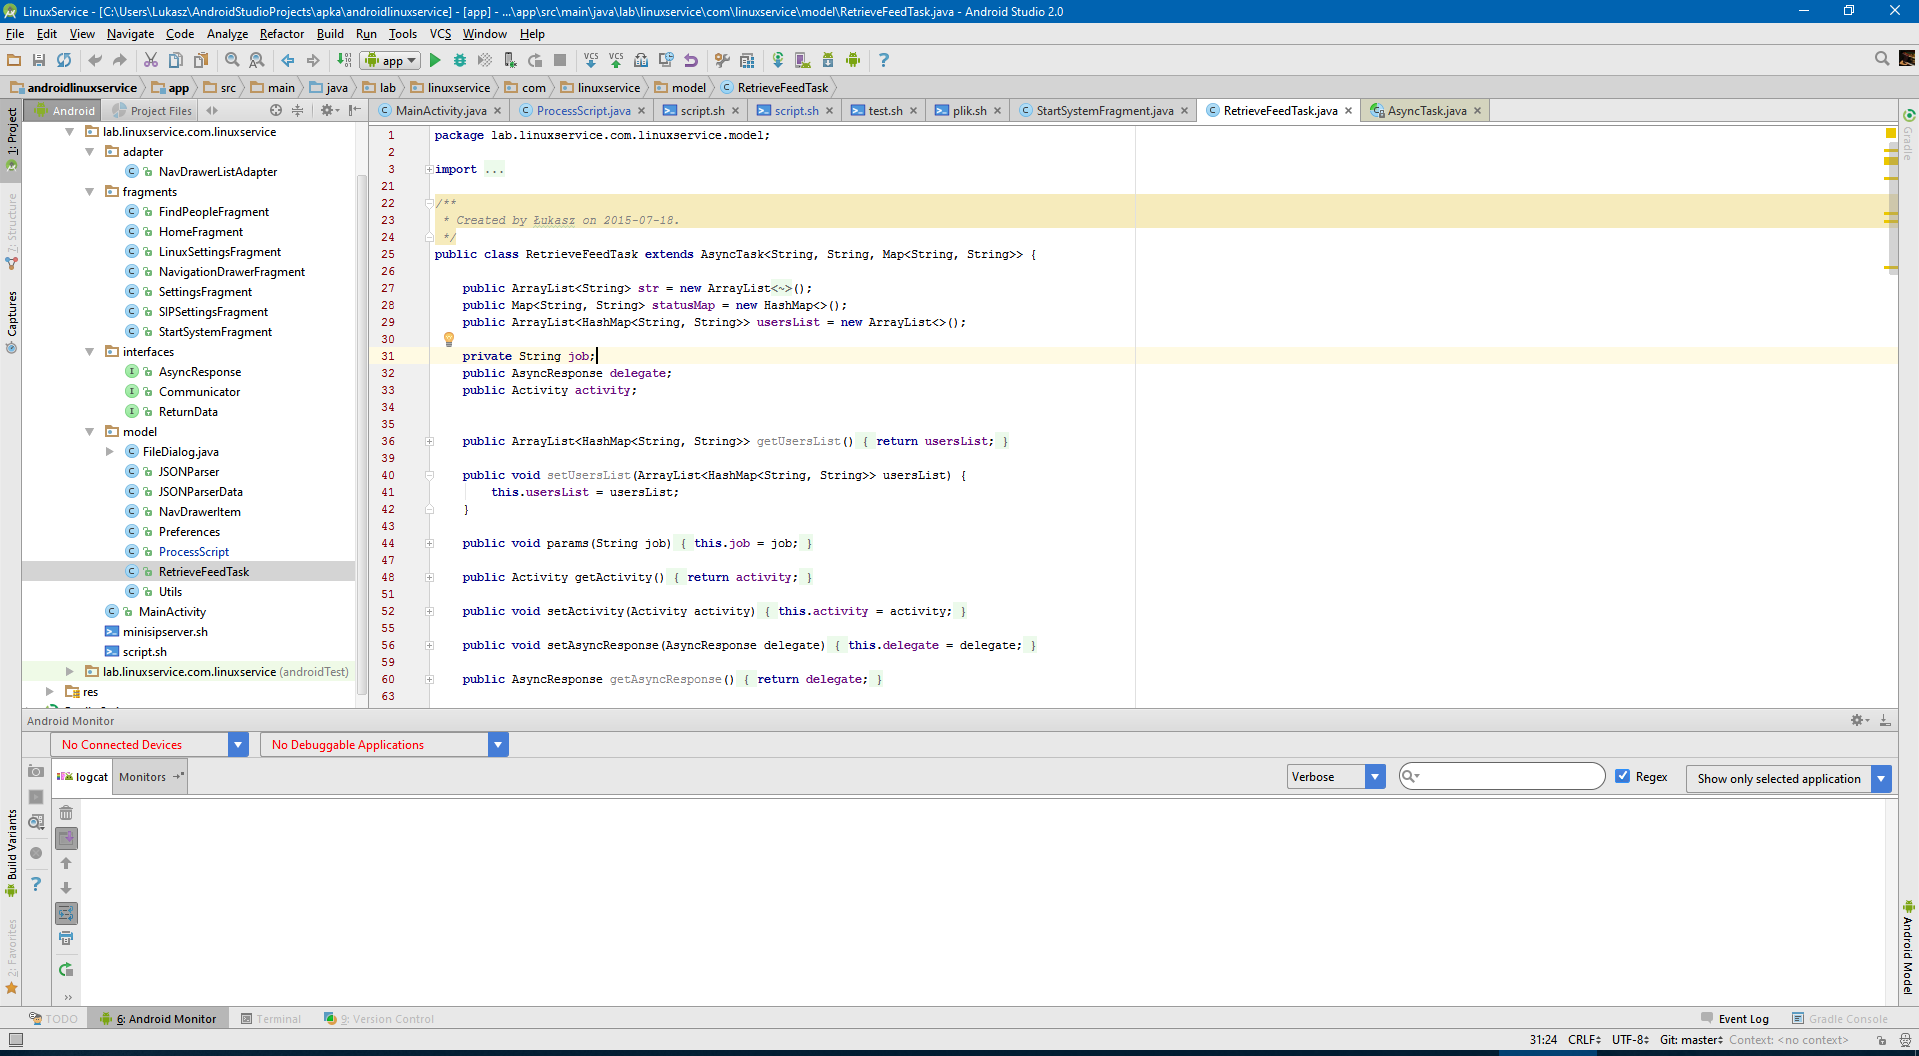
\includegraphics[width=1\linewidth]{androidstudio}
	\caption{Interfejs Android Studio}
	\label{fig:androidstudio}
\end{figure}
Za pomocą modułu SDK Manager można pobrać wersje systemu Android.

\begin{figure}[H]
	\centering
	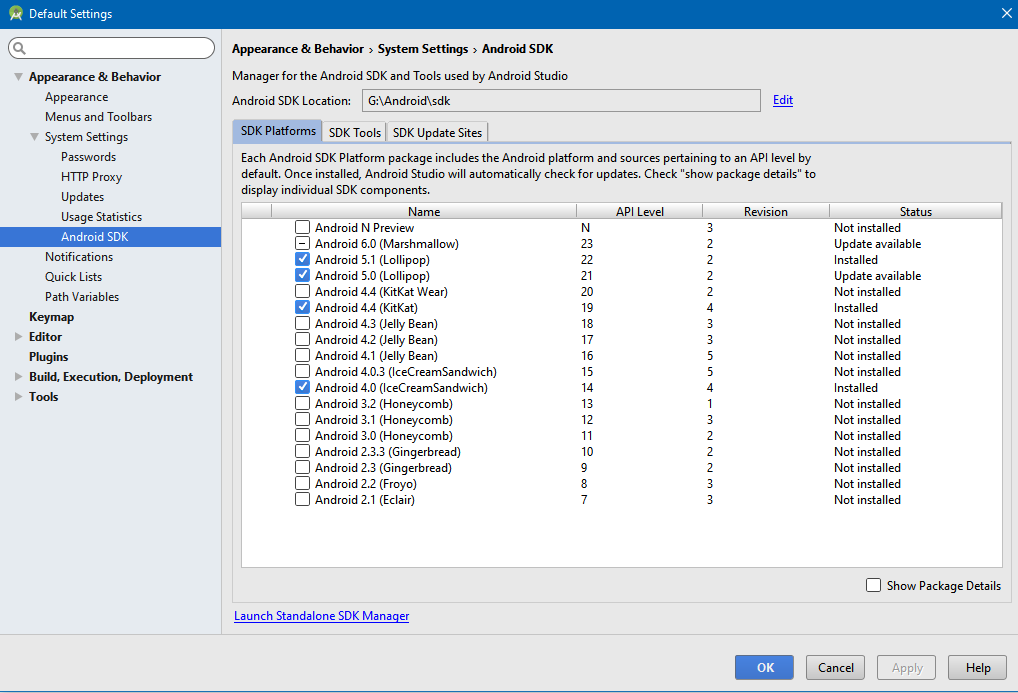
\includegraphics[width=1\linewidth]{sdkmenager}
	\caption{Menedżer pakietów SDK}
	\label{fig:sdkmenager}
\end{figure}
IDE oferuje graficzny edytor wyglądu aplikacji, który znacznie ułatwia pracę.
\begin{figure}[H]
	\centering
	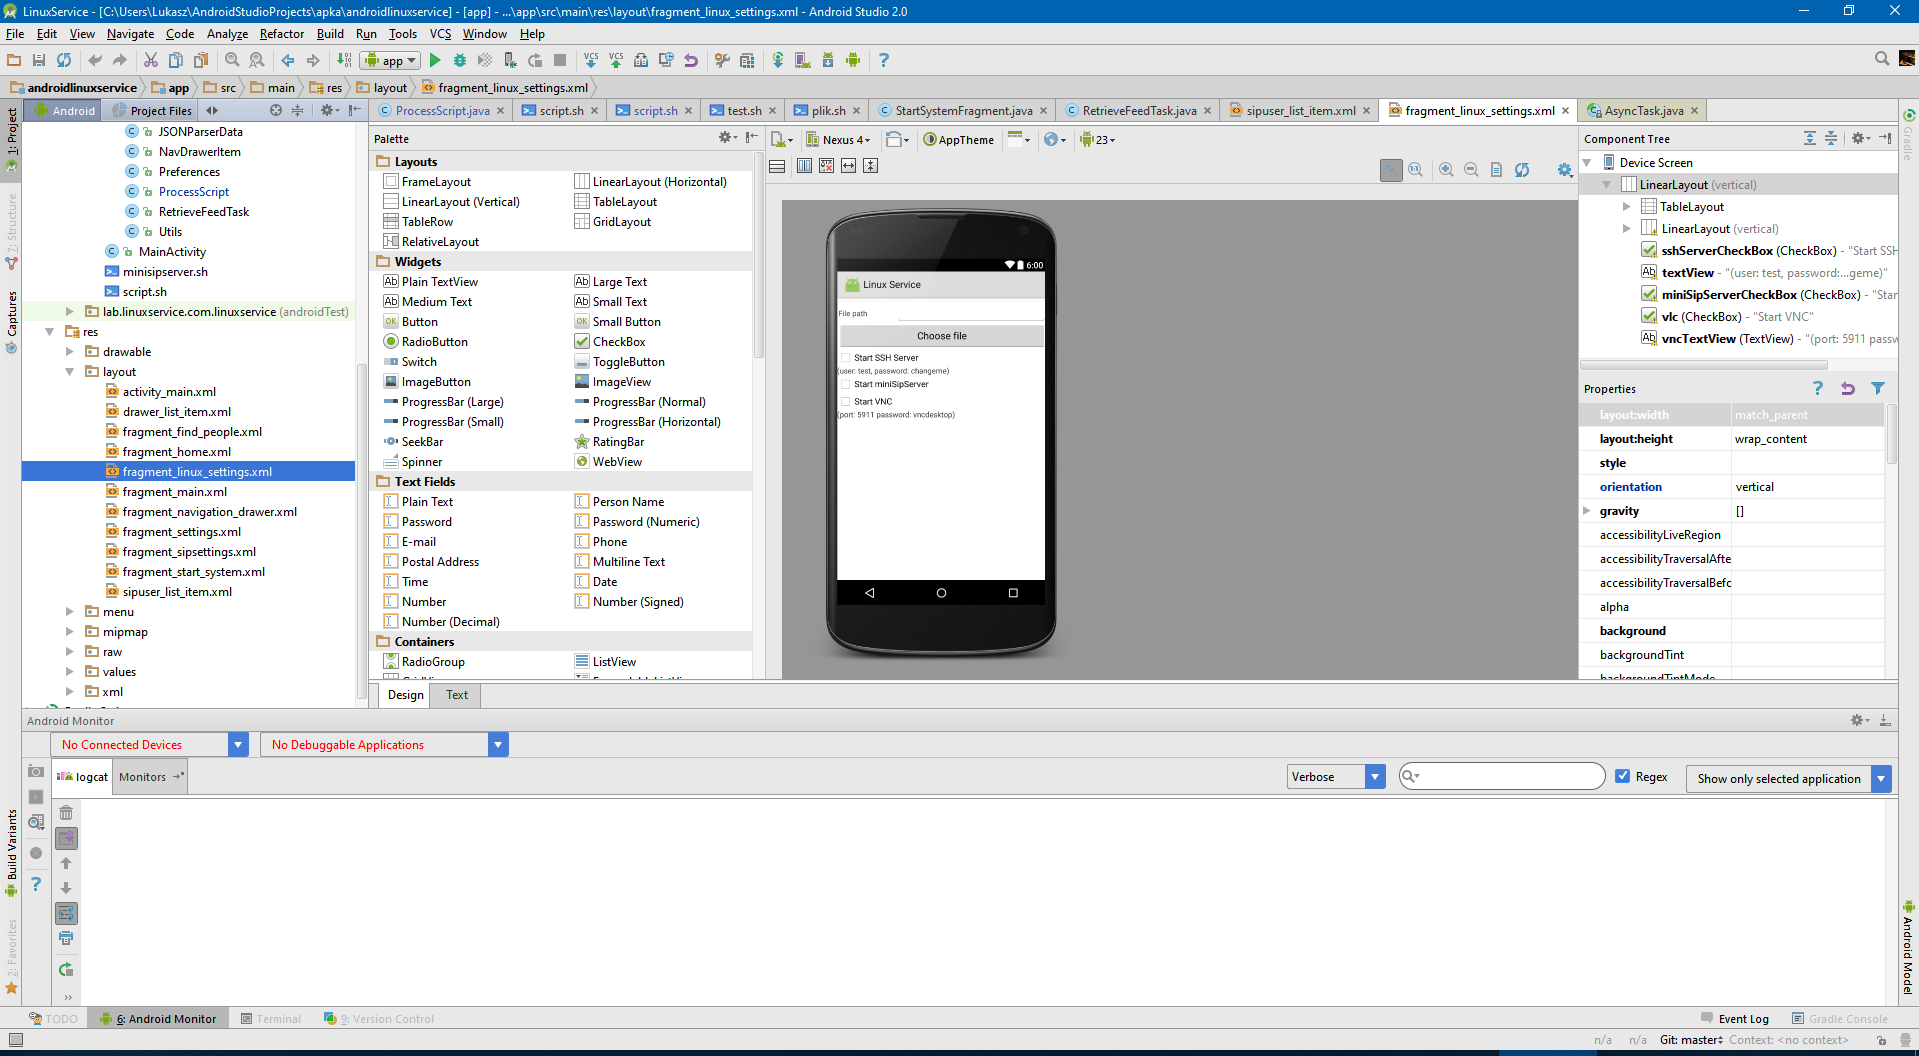
\includegraphics[width=1\linewidth]{widokprojektowy}
	\caption{Widok projektowy wyglądu aplikacji}
	\label{fig:widokprojektowy}
\end{figure}
\section{Kod źródłowy aplikacji i jej działanie}

Aplikacja została przygotowana z wykorzystaniem API na poziomie 22, które obsługuje system Andoird 5.1 Lollipop.

\subsection{Struktura klas aplikacji}

Diagramy zostały wygenerowane na podstawie napisanego kodu za pomocą wtyczki simpleUML Diagram w programie Android Studio. Struktura klas aplikacji przedstawia się następująco: 

\begin{figure}[H]
	\centering
	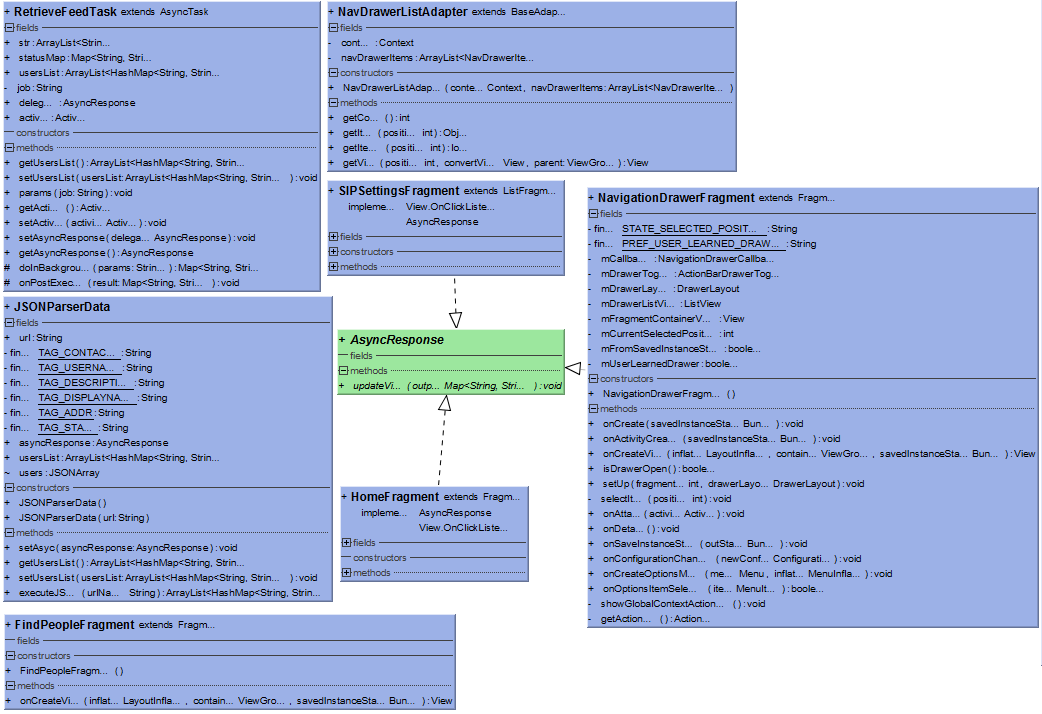
\includegraphics[width=1.1\linewidth]{uml1}
	\caption{Struktura klas aplikacji cz. 1}
	\label{fig:uml1}
\end{figure} 
\begin{figure}[H]
\centering
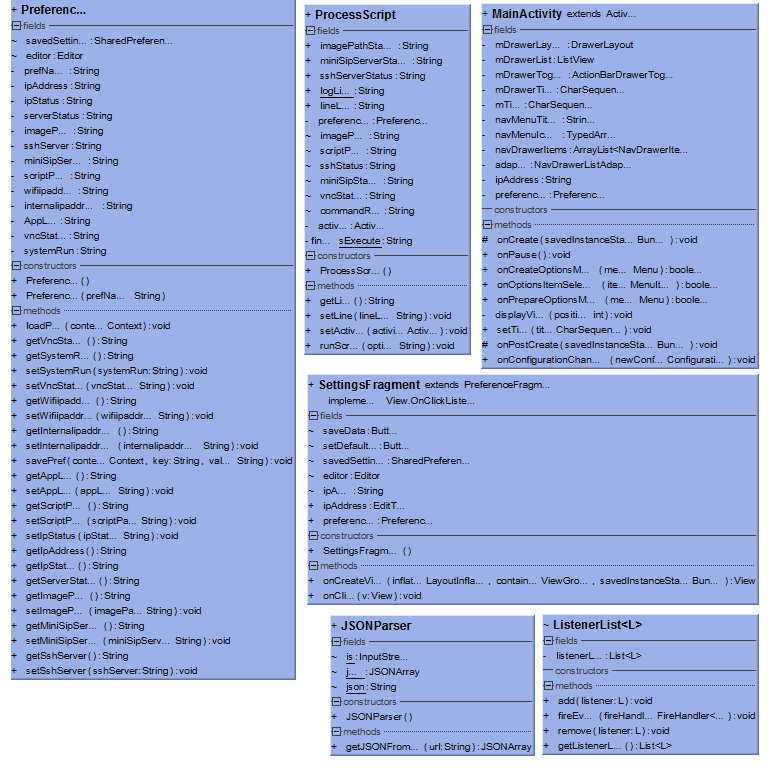
\includegraphics[width=1.1\linewidth]{uml2}
\caption{Struktura klas aplikacji cz. 2}
\label{fig:uml2}
\end{figure}
\begin{figure}[H]
\centering
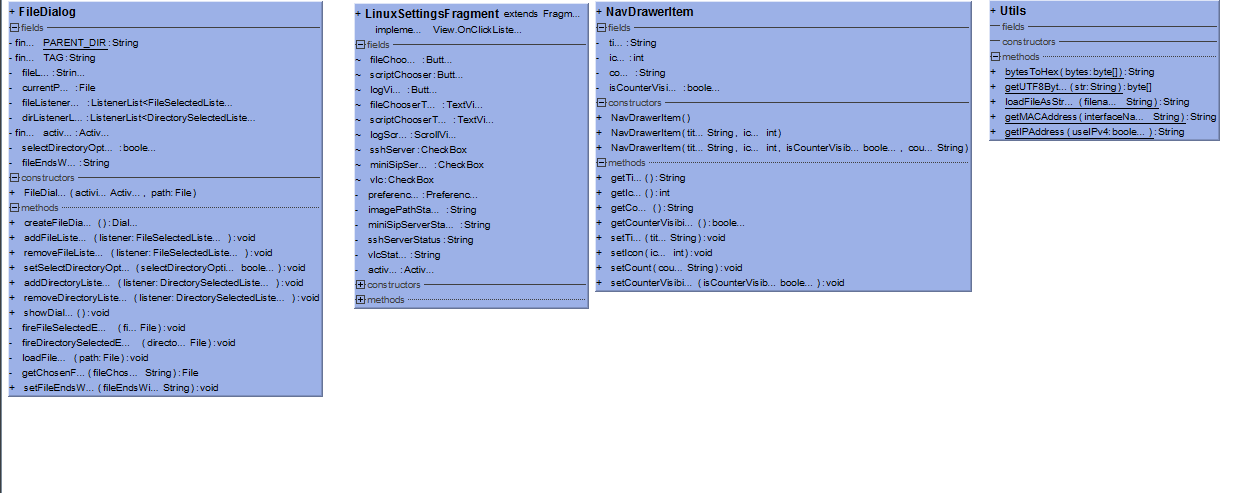
\includegraphics[width=1.1\linewidth]{uml3}
\caption{Struktura klas aplikacji cz. 3}
\label{fig:uml3}
\end{figure}

\newpage

\subsection{Interfejs aplikacji}
Interfejs aplikacji składa się z trzech części:

\begin{figure}[H]
\centering
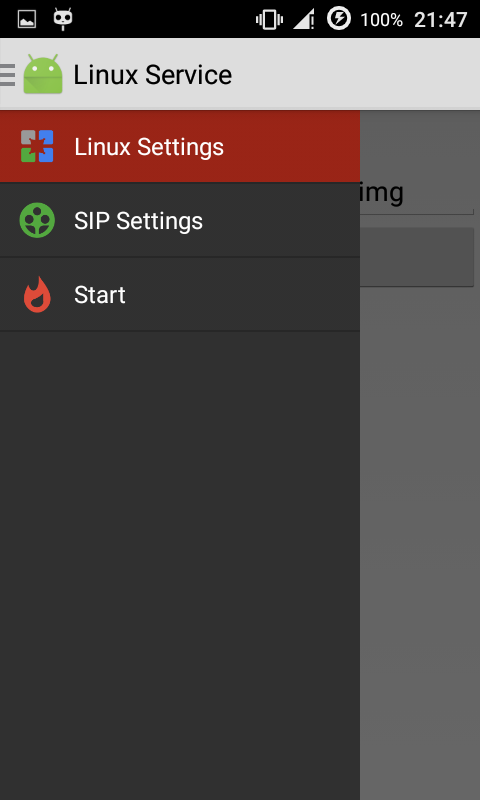
\includegraphics[width=0.5\linewidth]{Screenshot_2015-09-20-21-47-49}
\caption{Menu aplikacji}
\label{fig:Screenshot_2015-09-20-21-47-49}
\end{figure}


\begin{itemize}
	\item Linux Settings - zakładka umożliwia wybranie obrazu systemu, który ma być montowany. Plik wybieramy z okna dialogowego, w razie wybrania niepoprawnego pliku zostaniemy o tym poinformowani. Kolejno jest możliwość uruchomienia trzech usług: serwera SSH, serwera miniSipServer oraz serwera VNC Tightvnc. Wybrane opcje są zapamiętywane w pamięci programu i są wczytywane przy kolejnym uruchomieniu programu.
	
    \begin{figure}[H]
\centering
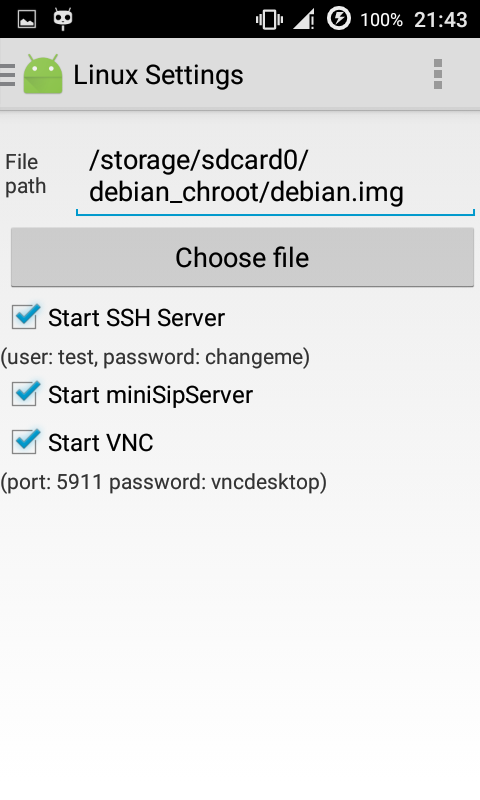
\includegraphics[width=0.5\linewidth]{Screenshot_2015-09-20-21-43-44}
\caption{Karta Linux Settings}
\label{fig:Screenshot_2015-09-20-21-43-44}
\end{figure}
\newpage
\item SIP Settings - zakładka umożliwia zarządzania serwerem miniSipServer. Do zarządzania wykorzystywane jest API, które oferuje miniSipServer. W tej części mamy dostęp do:
\begin{itemize}
\item dodania nowego użytkownika - Rysunek 3.10
\item wyświetlenie listy użytkowników - Rysunek 3.11
\item usunięcie użytkownika - Rysunek 3.11
\item jeżeli chcemy zarządzać serwerem miniSipServer, który nie jest uruchomiony na naszym urządzeniu możemy podać inny adres IP - Rysunek 3.12

\item dostęp do panelu administracyjnego poprzez przeglądarkę internetową.
\end{itemize}
    
\begin{figure}[H]
	\centering
	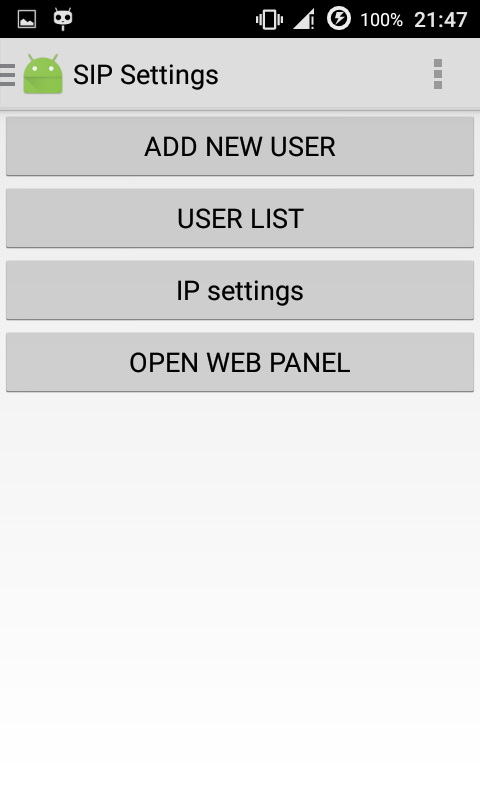
\includegraphics[width=0.5\linewidth]{Screenshot_2015-09-20-21-47-54}
	\caption{Karta SIP Settings}
	\label{fig:Screenshot_2015-09-20-21-47-54}
\end{figure}


\begin{figure}[H]
	\centering
 
	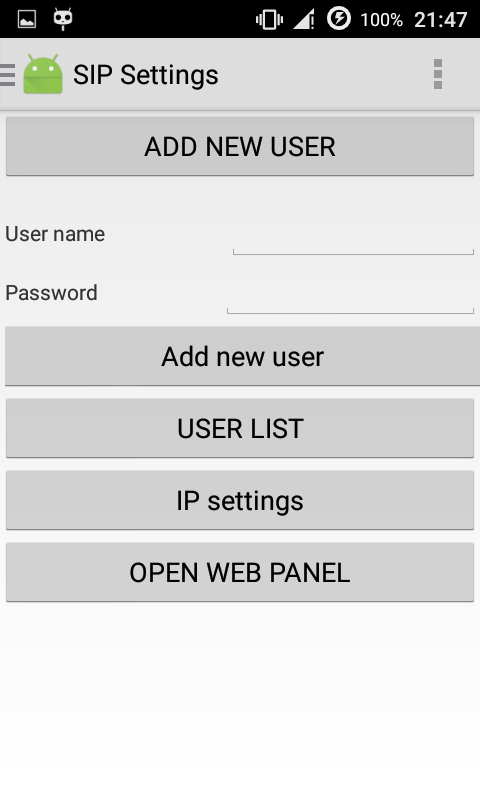
\includegraphics[width=0.4\linewidth]{Screenshot_2015-09-20-21-47-57}
	\caption{Folmularz dodawania nowego użytkownika}
	\label{fig:Screenshot_2015-09-20-21-47-57}
	\vspace{2cm}
		\centering
		\vspace{1cm}
		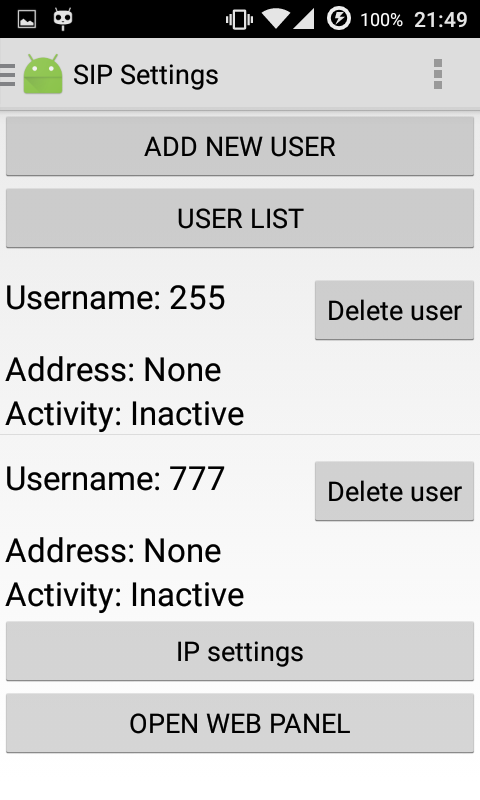
\includegraphics[width=0.4\linewidth]{Screenshot_2015-09-20-21-49-48}
		\caption{Lista użytkowników}
		\label{fig:Screenshot_2015-09-20-21-49-48}
\end{figure}


 


\begin{figure}[H]
 
		\centering
		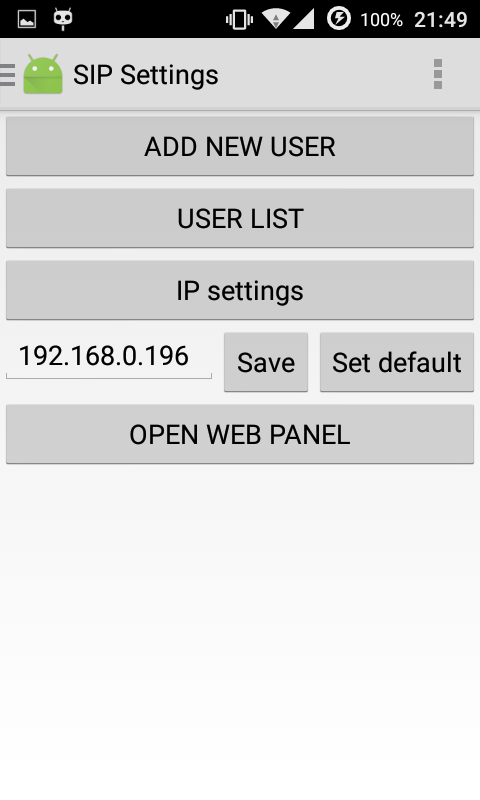
\includegraphics[width=0.4\linewidth]{Screenshot_2015-09-20-21-49-55}
		\caption{Ustawienia adresu IP}
		\label{fig:Screenshot_2015-09-20-21-49-55}
		\vspace{2cm}
	 
\end{figure}
\newpage	
\item Start - zakładka pozwala na uruchomienie systemu bądź jego zatrzymanie z dostępem do logu - Rysunek 3.13 

\begin{figure}[H]
	
		\centering
		
		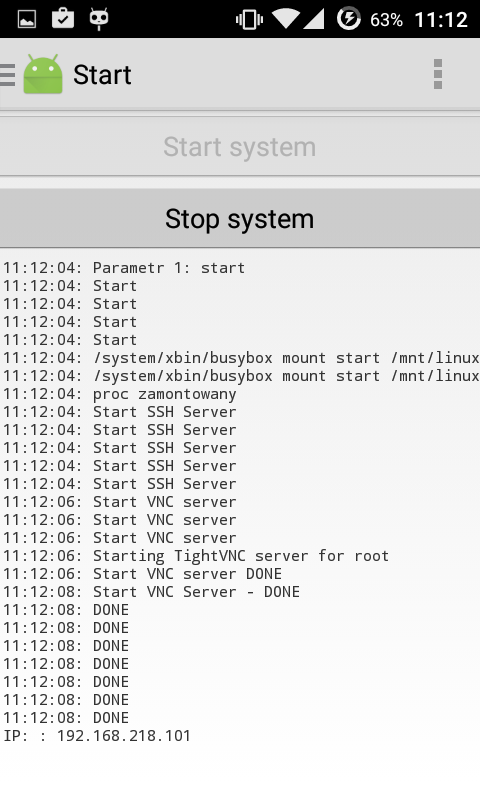
\includegraphics[width=0.4\linewidth]{Screenshot_2015-09-21-11-12-13}
		\caption{Start / Stop systemu}
		\label{fig:Screenshot_2015-09-21-11-12-13}
		\end{figure}
	
\end{itemize}

\subsection{Interfejs webowy serwera miniSipSerwer}

miniSipServer oferuje zarządzanie serwerem poprzez stronę internetową. Interfejs webowy jest dostępny od wersji 3.1. Razem ze startem serwera SIP startuje serwer HTPP, którego zadaniem jest umożliwienie dostępu do strony internetowej. Domyślnie miniSipServer dla serwera HTTP otwiera port TCP 8080. Po wpisaniu http://adresip:8080/ w przeglądarkę internetową wejdziemy na stronę umożliwiającą zarządzanie serwerem SIP.




\begin{figure}[H]
\centering
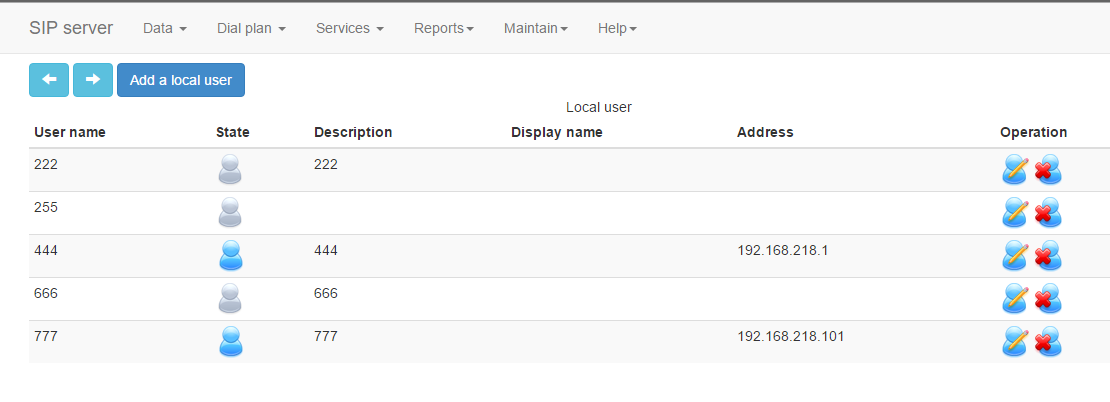
\includegraphics[width=1.1\linewidth]{sipweb}
\caption{Lista użytkowników w systemie}
\label{fig:sipweb}
\end{figure}




\clearpage
\afterpage{\null\newpage}
 

\chapter*{Zakończenie}
\addcontentsline{toc}{chapter}{Zakończenie}
Dostępne obecnie urządzenia mobilne bazujące na systemie Android to nie tylko aparaty służące do wykonywania rozmów telefonicznych czy pisania wiadomości tekstowych. Urządzenie daje nam wiele możliwości jeżeli wiemy jak je wykorzystać. Z telefonu komórkowego możemy zrobić dowolne urządzenie, może to być opracowany w pracy serwer telefonii SIP czy chociażby sniffer sieci Wi-Fi. Możliwości jakie daje nam oprogramowanie bazujące na systemie Linux jest bardzo duże. Rynek telefonii SIP rozwija się z każdym rokiem. Praktycznie każda większa firma powinna mieć własną sieć telefoniczną, a instalacja takiej sieci w cale nie musi oznaczać dużej inwestycji. 
\afterpage{\null\newpage}

\clearpage
\afterpage{\null\newpage}
 
\listoffigures
\addcontentsline{toc}{section}{Spis rysunków}


\begin{thebibliography}{9}
	
	\bibitem{lamport94}
	Marcin Bis,
	\emph{Linux w systemach Embedded, btc Warszawa 2011}
	
	\bibitem{lamport94}
	Karim Yaghmour,
	\emph{Embedded Android, O'Reilly 2013}
	
	
	\bibitem{lamport94}
	
	\emph{https://dug.net.pl/tekst/193/instalacja_debiana_metoda_debootstrap/
	}
	
	\bibitem{lamport94}
	
	\emph{http://androlinux.com/android-ubuntu-development/how-to-build-chroot-arm-ubuntu-images-for-android/ }     
	
	
	\bibitem{lamport94}
	
	\emph{http://androlinux.com/     }
	
	\bibitem{lamport94}
	
	\emph{http://ingvar.blog.redpill-linpro.com/2011/05/20/running-fedora-on-the-galaxy-s/ }
	
	\bibitem{lamport94}
	
	\emph{http://mitchtech.net/android-ubuntu-chroot/}
	
	\bibitem{lamport94}
	
	\emph{http://www.cyberciti.biz/faq/unix-linux-chroot-command-examples-usage-syntax/              
	}
	\bibitem{lamport94}
	
	\emph{https://www.kernel.org/doc/Documentation/filesystems/ramfs-rootfs-initramfs.txt }
	
	\bibitem{lamport94}
	
	\emph{http://linux.die.net/man/2/chroot}
	\bibitem{lamport94}
	
	\emph{http://linux.die.net/man/8/pivot_root}
	
	
	\bibitem{lamport94}
	
	\emph{http://students.mimuw.edu.pl/SO/Projekt04-05/temat4-g4/mikrokontrolery.htm}                                
	\bibitem{lamport94}
	
	\emph{https://github.com/meefik/linuxdeploy}  
	\bibitem{lamport94}
	
	\emph{http://www.g-loaded.eu/2008/01/28/how-to-extract-rpm-or-deb-packages/}                                                                                                                 
\end{thebibliography} 


\end{document}
